\chapter{SIMC}

%------------------
% TODO: move most of this to chap 4 or an appendix?

% The general structure of SIMC's simulation for (quasi)elastic
% scattering is described below.
% \begin{enumerate}
%     \item Initialization
%     \begin{itemize}
%         \item Choose a reaction and final state
%         % \item Disable/enable implementation of (or correction for) raster, eloss ...
%     \end{itemize}

%     \item Event Generation
%     \begin{itemize}
%         \item Generate an event vertex based on target geometry,
%               beam width, beam raster, and beam energy
%         \item Generate $\theta_e$, $\phi_e$, $p_e$,
%                        $\theta_p$, $\phi_p$, $p_p$
%     \end{itemize}

%     \item Event Propagation
%     \begin{itemize}
%         \item Adjust event for radiative effects, Coulomb corrections, particle decays, etc.
%         \item Propagate particles through spectrometers using COSY models,
%               applying energy loss and multiple scattering in the target and
%               detectors.
%     \end{itemize}

%     \item Event Reconstruction
%     \begin{itemize}
%         \item Fit tracks in the focal plane
%         \item Reconstruct target variables $\delta$, $x'_{tar}$, $y'_{tar}$, $y_{tar}$
%     \end{itemize}

%     \item Normalization and Saving to Disk
%     \begin{itemize}
%         \item Calculate $E_m$ and $\vec{p}_m$ if simulating quasielastic scattering
%         \item Calculate per-event weight from spectral function, cross section,
%               radiative correction weight, and event generation weight.
%         \item Calculate normalization factor \textit{normfac} from luminosity,
%               phase space factors, and total number of events generated.
%         \item Save per-event physics quantities and weights in an Ntuple in a
%               PAW HBOOK.
%     \end{itemize}
% \end{enumerate}

% \textit{SIMC}'s output \texttt{.hbook} files can be converted to \texttt{.root}
% files for analysis alongside \textit{hcana} output using the utility
% \textit{h2root}.

% Good note explaining normfac
% https://hallaweb.jlab.org/12GeV/experiment/E12-07-108/Publications/Technical/Spectrometer/SIMC/simc_extra.pdf
% Gaskell/Arrington talk on simc
% https://hallaweb.jlab.org/collab/meeting/2009-winter/talks/Analysis%20Workshop%20--%20Dec%2014/simc_overview.pdf

\section{Spectral Functions}

The spectral functions used in SIMC are based on the independent particle shell
model (IPSM), which assumes nucleons occupy shells with quantum numbers $n$,
$l$, $j$, similar to the model of electron orbitals in atomic physics.
% preetty good slides
% http://indico.ictp.it/event/7641/session/21/contribution/46/material/0/0.pdf
In this model, the spectral function can be factored into a sum of per-shell
energy and momentum distributions
\begin{equation}
    S(E_m,\vec{p}_m) = \sum_i N_i \norm{\varphi_i(\vec{p})}^2 L_i(E_m)
\end{equation}
where $N_i$ is the occupation number of the $i$th shell,
$\varphi_i(\vec{p})$ is the bound state wavefunction,
and $L_i(E_m)$ is an energy profile.


% TODO: Give one of these Ls a tilde or prime to account for normalization?
The energy profile of each nuclear shell $i$ with binding energy $E_i$ is
given by a Lorentzian with finite width $\Gamma_i$ that accounts for the finite
lifetime of the one-hole state.
\begin{equation}
    L_i(E) = \frac{1}{\pi} \frac{\Gamma_i/2}{(E-E_i)^2 + \Gamma_i^2/4}
\end{equation}

The separation energy $E$ cannot be less than the minimum proton removal
energy $E_{min}=m_p + m_{A-1} - m_A$, so these profiles are cut off below
$E_min$ and normalized to ensure the spectroscopic sum rule,
Equation~\ref{eqn:spectroscopic_sum_rule}, is obeyed.
\begin{equation}
    L_i(E) =
    \begin{cases}
        L_i(E) / \int^{\infty}_{E_{min}} L_i(E) dE & \text{if $E \geq E_{min}$} \\
        0 & \text{if $E<E_{min}$}
    \end{cases}
\end{equation}


The wavefunctions $\varphi_i(\vec{p})$ are Fourier transforms of solutions
$\psi(\vec{r})$ to the Schroedinger equation with a potential given by the sum
of a
Woods-Saxon potential $-V_0 f(\vec{r})$,
Coulomb potential $V_C(r)$,
and spin-orbit coupling,
\begin{equation}
    V(\vec{r}) = - V_{0} f(r)
                 + V_{C}(r)
                 + V_{SO} \left(\frac{\hbar}{m_\pi c}\right)^{2}
                          \frac{2}{r} \frac{df}{dr}
                          \vec{l}\cdot\vec{s}
\end{equation}

The Woods-Saxon potential is characterized by
depth $V_0$,
radius $R_0=r_0(A-1)^{1/3}$, and
diffuseness $a$
parameters and a form given by a Fermi-Dirac distribution
\begin{equation}
    f(r) = \frac{1}{1+e^{\frac{r-R_0}{a}}}
\end{equation}
The Coulomb potential is that of a uniform sphere of radius
$R_c=r_c(A-1)^{1/3}$.


The model parameters were obtained from fits to the Saclay
measurements~\cite{Mougey_1976, Frullani_1984} of the ${}^{12}C$ spectral
functions.
The wavefunctions were obtained using the method described in
Ref~\cite{Giusti_1988, Giusti_1987, Blok_1991}.
% TODO: clarify: is this still the DWEEPY stuff others describe?
% TODO: table of relevant parameters?


Short range nucleon-nucleon correlations push protons to higher missing energy
and momentum than accounted for by the IPSM.
Without correcting for this, simulated yields would be artificially large.
Assuming this leads to a uniform suppression of the spectral function below the
Fermi momentum, the spectral functions can be corrected by a constant factor,
assuming one consistently works in the same volume $V_m$ of $(E_m,\vec{p}_m)$ phase
space.
Given spectral functions $S_{SRC}$,that include the effects of short range
correlations, the correction is given by
\begin{equation}
    \frac{\int_{V_m} S_{IPSM}(E_m,\vec{p}_m) dE_m d^3p_m}
         {\int_{V_m} S_{SRC} (E_m,\vec{p}_m) dE_m d^3p_m}
\end{equation}
% DD: A more realistic estimate of the SRC correction would have different
% values for the p and s-shell with the overall correction averaging to 12%

\section{Coulomb Corrections}
Coulomb distortions of the PWIA model arise from electromagnetic interactions
between the beam electron and target nucleus, modifying the momentum transfer
and incoming/outgoing momenta of the electron.


The energy required to bring an electron from infinity to a position $\vec{r}$
inside a nucleus with $Z-1$ protons is
\begin{equation}
    \Delta E(\vec{r})=f_{C}(|\vec{r}|)\left[\alpha \frac{(Z-1)}{R_{0}}\right]
\end{equation}
where
$\vec{r}=0$ is the center of the nucleus,
$\alpha$ is the fine structure constant,
and
$R_0=1.1 A^{1/3}+0.86 A^{-1/3}$ is the radius of the nucleus.


\textit{SIMC} uses the prescription described in Ref~\cite{Aste_2005}, which
takes this energy to be
\begin{equation}
    \Delta E = \frac{f(Z-1)\alpha}{R_0}
\end{equation}
where the factor $f$ is of order 1; SIMC uses $f=1.125$.


Assuming the incoming electron is not deflected, its initial momentum at the
interaction vertex becomes
\begin{equation}
    (\vec{p}_e)_v = \vec{p}_e(1 + \Delta E / p_e)
\end{equation}
This value is used to calculate the momentum transfer
\begin{equation}
    \vec{q} = (\vec{p'}_e)_v - (\vec{p}_e)_v
\end{equation}
and opposite correction is applied to the outgoing electron momentum,
\begin{equation}
    \vec{p}_e = (\vec{p'}_e)(1 - \Delta E / (p'_e)_v)
\end{equation}

% \section{Final State Interactions}
% TODO: FSI in SIMC


% \section{Pauli Blocking}
% TODO: write Pauli blocking section? I don't think we actually use it in QE simulation?
% Basic idea:
% In Fermi gas, all states below k_F are filled.
% When a pion is produced in A(e,e'pi+)n, the recoil neutron might not have
% anywhere to go!
% So occupation levels are smoothed out.
% SIMC uses Fantoni 1984 data for this.

\section{Radiative Corrections}
The method for radiative corrections in \textit{SIMC} is based on the work of
Mo and Tsai~\cite{Mo_1969}.
The full derivation by Makins et. al~\cite{Ent_2001, Makins_1994} for
coincidence elastic and quasielastic scattering done is quite length.
What follows in this section is an overview of the main results.
In brief, \textit{SIMC} calculates vertex corrections and the energy radiated
as internal and external Bremsstrahlung, modifies the simulated particles'
vertex 4-momenta accordingly, and applies a weight to the event.

\subsection{Internal Bremsstrahlung}
The cross section for scattering an electron into a solid angle $d\Omega_e$
accompanied by the emission of a single photon is
\begin{align}
    \frac{d\sigma}{d\Omega_e d^3\omega} &=
        \left.\frac{d \sigma^{(1)}}{d \Omega_{e}}\right|_{e p}
        \frac{-\alpha}{4 \pi^{2} (\omega^{0})^2}
        \left[ \frac{k'}{\omega \cdot k'} -
                \frac{p'}{\omega \cdot p'} -
               \frac{k}{\omega \cdot k} +
               \frac{p}{\omega \cdot p}
        \right]^2 \\
     &= \left. \frac{d\sigma^{(1)}}{d\Omega_e}\right|_{ep}
         \frac{A(\hat{\omega})}{\omega^0}
\end{align}

where $\left. \frac{d\sigma^{(1)}}{d\Omega_e}\right|_{ep}$ is the single-photon
exchange $ep$ cross section,
and $A(\hat{\omega})$ is the angular distribution of single photon Bremsstrahlung.
The kinematic terms on the right hand side come from the
amplitudes given by the Feynman diagrams in Fig~\ref{fig:single_photon_brem_feynman}

\begin{figure}[!h]
    \centering
    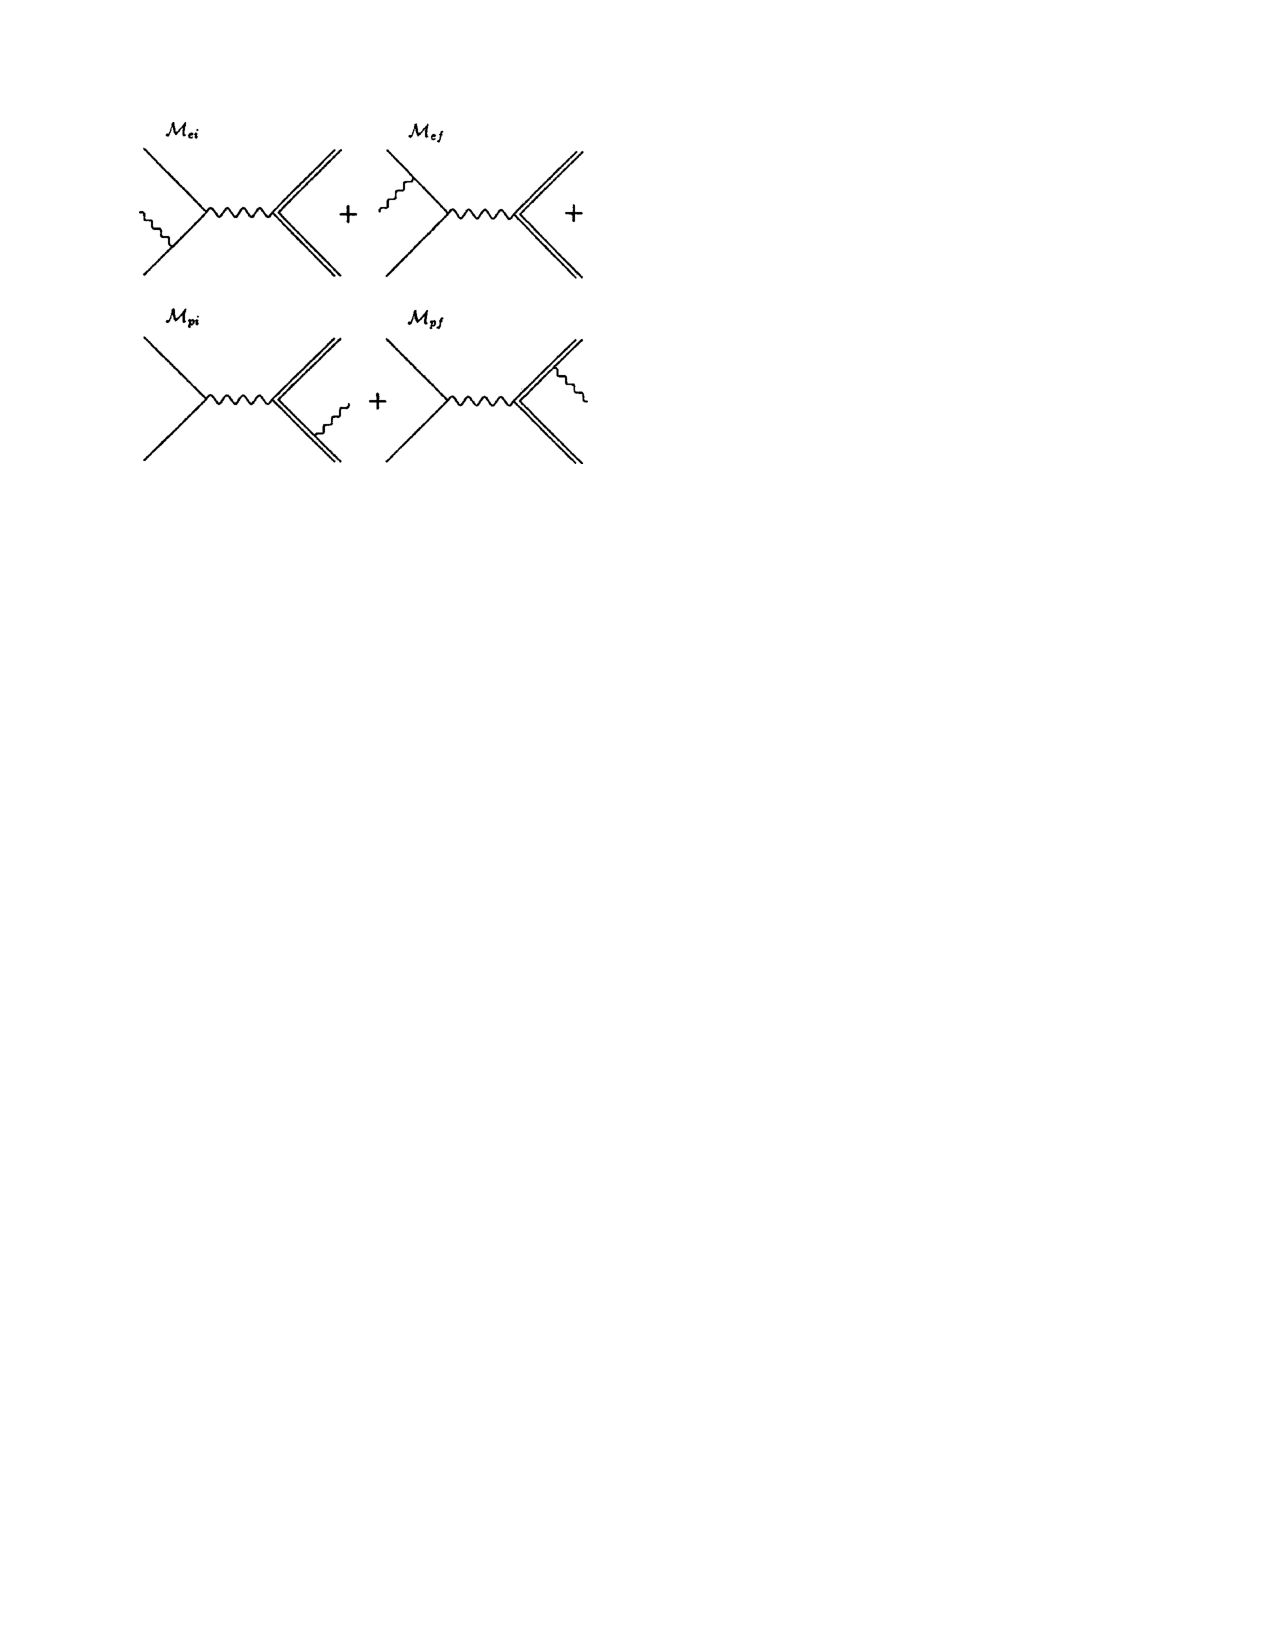
\includegraphics[width=0.7\textwidth]{chap1/single_photon_brem_feynman.pdf}
    \caption{
             Figure reproduced from Ref~\cite{Ent_2001}.
             }
    \label{fig:single_photon_brem_feynman}
\end{figure}

% TODO: remove some of this derivation stuff so we only have main results
Let
\begin{equation}
    B(p_i, p_j, \Delta E_m) = \int_0^{\Delta E_m} d^3 \omega
    \frac{1}{8\pi^2\omega^0}
    \frac{p_i \cdot p_j}{(\omega \cdot p_i)(\omega \cdot p_j)}
\end{equation}
and
\begin{equation}
    \lambda = \int d\Omega_\gamma A(\hat{\omega})
\end{equation}

Allowing the emission of multiple Bremsstrahlung photons, with a total energy
$E_{tot}$,

\begin{equation}
    \frac{d\sigma}{d\Omega_e d^3\omega} =
        \left.\frac{d \sigma^{(1)}}{d \Omega_{e}}\right|_{e p}
        (1-\sigma_{hard})
        (-\delta'_{soft}(E_{tot})
        e^{-\delta_{soft}(E_{tot})}
        F(\lambda)
\end{equation}

where $F(\lambda)=\frac{e^{-C\lambda}}{\Gamma(1+\lambda)}$ and $C$ is the
Euler-Mascheroni constant.
% TODO: clarify: is \delta'_{soft}(E) = \frac{d\delta_{soft}(E)}{dE}?


The contribution from one photon Bremsstrahlung is
\begin{equation}
    \delta_{soft}(\Delta E_m) = 2\alpha \sum_{i,j} \Theta(p_i) \Theta(p_j)
                                                   \bar{B}(p_i,p_j,\Delta E_m)
\end{equation}
where $\bar{B}(p_i,p_j,\Delta E_m)$ is $B(p_i,p_j,\Delta E_m)$ without the
infrared divergent term
$p_i$ is one of $k,k',p,p'$
and
$\Theta(p_i)$ is the sign function.

The contribution from one-loop diagrams is
\begin{equation}
    \delta_{hard} = 2\alpha
                    \left[
                        -\frac{3}{4\pi}\log\left(\frac{-q^2}{m_e^2}\right)
                        + \frac{1}{\pi}
                        - \sum_i \delta^{vp}_i(q^2)
                    \right]
\end{equation}
where
\begin{equation}
    \delta^{vp}_i = \frac{1}{3 \pi}
                        \left(
                            -\frac{5}{3} - \frac{4 m_{i}^{2}}{q^{2}} +
                            \left(1+\frac{2 m_{i}^{2}}{q^{2}}\right)
                            \sqrt{1-\frac{4 m_{i}^{2}}{q^{2}}}
                            \log \left[\frac{\sqrt{1-\frac{4 m_{i}^{2}}{q^{2}}}+1}
                                            {\sqrt{1-\frac{4 m_{i}^{2}}{q^{2}}}-1}
                                 \right]
                        \right)
\end{equation}
is the vacuum polarization correction due to flavor $i$ of leptons and light quarks of flavor $i$.

\begin{figure}[!h]
    \centering
    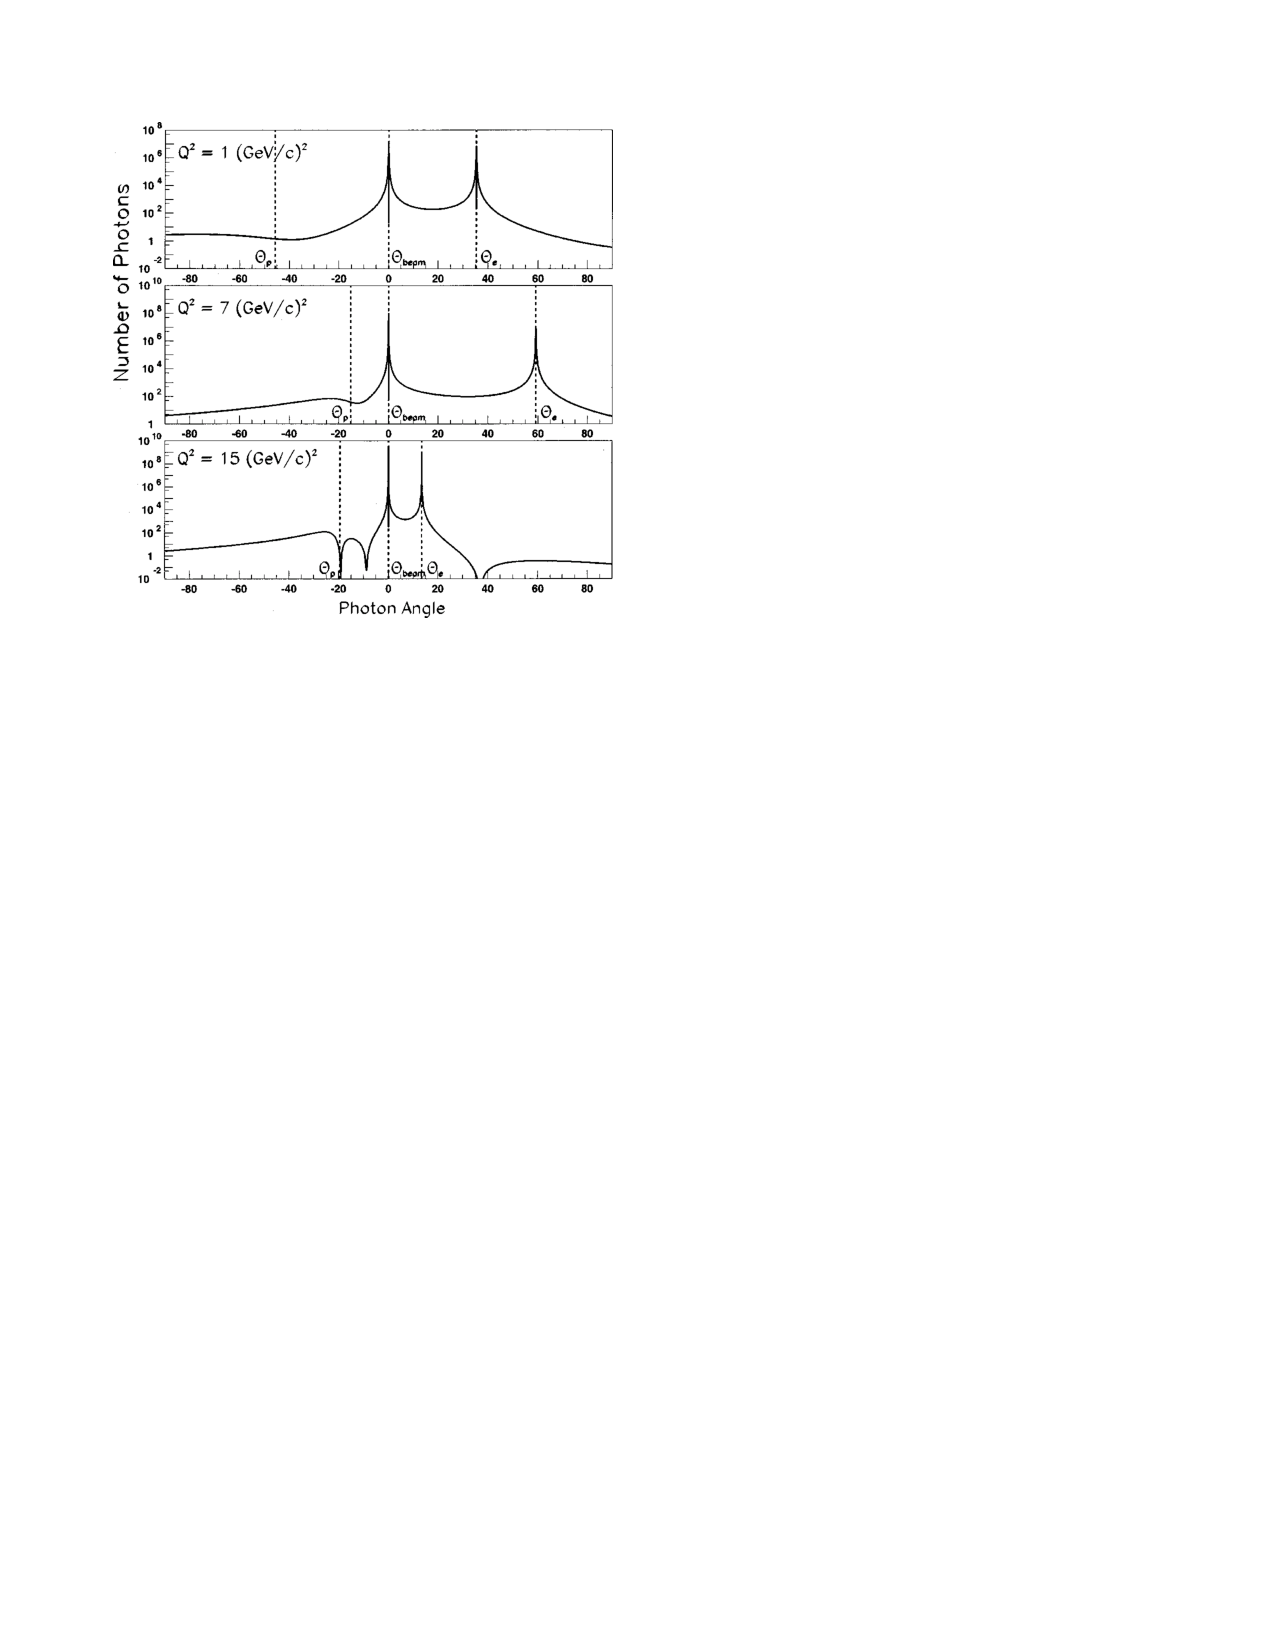
\includegraphics[width=0.7\textwidth]{chap1/single_photon_angular_distribution.pdf}
    \caption{The angular distribution of first order single photon
             Bremmstrahlung for three values of momentum transfer $Q^2$.
             The photon angle, given in degrees, is measured with respect to
             the direction of the incoming beam electron.
             The directions $\theta_e$ and $theta_p$ of the scattered electron
             and proton are indicated by dotted lines.
             Figure reproduced from Ref~\cite{Ent_2001}.
             }
    \label{fig:single_photon_angular_distribution}
\end{figure}

As shown in Fig~\ref{fig:single_photon_angular_distribution}, the single
photon angular distribution is peaked around the directions of the incoming and
outgoing electron, and this focus increases with momentum transfer $Q^2$.
A broad peak in the direction of the scattered proton also becomes more defined
with increasing $Q^2$.
The \textit{peaking approximation} consists of dividing the total energy
radiated in Bremmstrahlung into three photons of energy $E_e$, $E_{e'}$, and
$E_{p'}$ that travel in the directions
$\hat{k}$ of the incoming electron,
$\hat{k}'$ of the outgoing electron,
and
$\hat{p}'$ of the outgoing proton.
The angular distribution $A(\hat{\omega})$ then becomes
\begin{equation}
    A_{peaking}(\hat{\omega}) = \lambda_{e}  \delta(\hat{\omega}-\hat{k}) +
                                \lambda_{e'} \delta(\hat{\omega}-\hat{k}') +
                                \lambda_{p'} \delta(\hat{\omega}-\hat{p}')
\end{equation}
The form of these $\lambda_i$ terms can be found by breaking up the angular
distribution $A(\hat{\omega})$ into three terms---one due to electron, one
due to the proton, and one with the cross terms

\begin{align}
    A(\hat{\omega}) = -\frac{\alpha(\omega^0)^2}{4\pi^{2}}
                        &\left[\left(\frac{k^{\prime}}{\omega \cdot k^{\prime}}-\frac{k}{\omega \cdot k}\right)^{2}
                        + \left(\frac{p^{\prime}}{\omega \cdot p^{\prime}}-\frac{p}{\omega \cdot p}\right)^{2}\right.\nonumber\\
                        &\left.-2\left(\frac{k^{\prime}}{\omega \cdot k^{\prime}}-\frac{k}{\omega \cdot k}\right)
                        \left(\frac{p^{\prime}}{\omega \cdot p^{\prime}}-\frac{p}{\omega \cdot p}\right) \right]
\end{align}

By expanding each of these terms in the polar coordinate $\theta$,
making approximations about their asymptotic behavior near and away from the peaks,
and finally integrating them, one can distribute their contents among the three
directions
\begin{align}
    \lambda_e    &= \frac{\alpha}{\pi}\left[\log\left(\frac{4k^2}{m_e^2}\right) +
                                        2\log\left(\frac{k}{k'}\right) +
                                        \log\left(\frac{1-cos\theta_e}{2}\right)
                                        -1\right] \\
    \lambda_{e'} &= \frac{\alpha}{\pi}\left[\log\left(\frac{4k'^2}{m_e^2}\right) +
                                        2\log\left(\frac{k}{k'}\right) +
                                        \log\left(\frac{1-cos\theta_e}{2}\right)
                                        -1\right] \\
    \lambda_{p'} &= \frac{\alpha}{\pi}
                  \left[
                      \frac{p'^0}{|\vec{p}|}
                      \log\left(\frac{p'^0+|\vec{p}|}
                                     {p'^0-|\vec{p}|}\right)
                      - 2
                  \right]
\end{align}

Generalizing to multiphoton Bremsstrahlung,
\begin{align}
    \frac{d\sigma}{d\Omega_e dE_e dE_{e'} dE_{p'}} &= \left. \frac{d\sigma^{(1)}}{d\Omega_e}\right|_{ep} \left(1-\delta_{hard}\right) \\
    &\times\frac{\lambda_e \lambda_{e'} \lambda_{p'}} {\left(kk'\right)^{\lambda_e/2} \left(kk'\right)^{\lambda_{e'}/2} \left(m_p p'^0\right)^{\lambda_{p'}/2}} \\
    &\times\frac{1}{E_{e}^{1-\lambda_{e}} E_{e'}^{1-\lambda_{e'}} E_{p'}^{1-\lambda_{p'}}}
\end{align}

\subsection{External Bremsstrahlung}
% our flags:
% rad_flag = 0; "use best available formulas, generate in (ntail,Egamma) basis"
% extrad_flag = 2; "use BASIC ext rad formulas x phi"
External Bremsstrahlung refers to the emission of photons in the fields of
nuclei other than the nucleus participating in the primary scattering.
The proton emits a negligible amount of such radiation, but the electron will
experience these losses as it travels through various materials\footnote{
SIMC calculates external Bremsstrahlung for the region between the target
chamber entrance window and the spectrometer entrance windows.
Energy loss and multiple scattering are the dominant corrections in the magnets
and detectors.}

Early~\cite{Early_1973} provides a numerical solution for the probability that
an electron with momentum $k$ radiates a total energy $E^{ext}$ while traveling
through $t$ radiation lengths of material with atomic number Z,
\begin{equation}
    \frac{1}{\Gamma(1+bt)}
    \frac{bt}{E^{ext}}
    \left(\frac{E^{ext}}{k}\right)^{bt}
    \Phi^{ext}\left(\frac{E^{ext}}{k}\right)
\end{equation}
where $b$ is a parameter expressing the $Z$ dependence,
\begin{equation}
    b = \frac{1}{9}\left(12 + \frac{Z+1}{ZL_1+L_2}\right)
\end{equation}
where
$L_1 = \ln{184.15} - \frac{1}{3} \ln Z$
and
$L_2 = \ln{1194} - \frac{2}{3} \ln Z$.
The function $\Phi^{ext}$ is a correction for large photon energies.
For the incoming electron, \textit{SIMC} uses the approximate form
\begin{equation}
    \Phi^{ext}_e\left(\frac{E_e}{k}\right) = 1 - \frac{bt}{bt-\lambda_e}\frac{E_e}{k}
\end{equation}


\textit{SIMC} combines the internal and external Bremsstrahlung into three
photon energies $E_e$, $E_{e'}$, and $E_{p'}$
\begin{align}
\frac{d\sigma}{d\Omega_{e} dE_{e} dE_{e'} dE_{p'}} =&\left.\frac{d\sigma}{d\Omega_{e}}\right|_{ep} \left(1-\delta_{hard}\right) \\
    &\times \frac{1}{\Gamma\left(1+b t_{e}\right)}  \frac{bt_{e}  + \lambda_{e}} {k^{bt_{e}} (kk')^{\lambda_{e}/2}}  \frac{1}{E_{e}^{1 -\lambda_{e} -bt_{e}}} \\
    &\times \frac{1}{\Gamma\left(1+b t_{e'}\right)} \frac{bt_{e'} + \lambda_{e'}}{k^{bt_{e'}}(kk')^{\lambda_{e'}/2}} \frac{1}{E_{e'}^{1-\lambda_{e'}-bt_{e'}}} \\
    &\times \frac{\lambda_{p'}}{(m_p p')^{\lambda_{p'}/2}} \frac{1}{E_{p'}^{1-\lambda_{p'}}}
\end{align}

Using the energy distributions contained in this expression,
\textit{SIMC} generates the radiated energy based on the limits
$E_{min}$ and $E_{max}$
imposed by
the model spectral functions,
spectrometer acceptances,
and randomly generated initial and final 4-momenta of particles participating
in scattering.
These energies are then subtracted from the particles' vertex energies.


Then, \textit{SIMC} generates a weight $W^{event}_{rad}$ for the event based on the
probabilities of emitting energies $E_i$, where $i$ is one of $e$, $e'$, and
$p'$.
The first contribution to this weight,
$W^{soft}_{rad}=W^{e}_{rad}W^{e'}_{rad}W^{p'}_{rad}$, is due to Bremsstrahlung,
where
\begin{equation}
    W^{e}_{rad} = \frac{1}{\Gamma(1+bt_{e})} \frac{1}{k^{bt_{e}}(kk')^{\lambda_{e}/2}}
                \left((E^{e}_{max})^{bt+\lambda_{e}}-(E^{e}_{max})^{bt+\lambda_{e}}\right)
\end{equation}
\begin{equation}
    W^{e'}_{rad} = \frac{1}{\Gamma(1+bt_{e'})} \frac{1}{k^{bt_{e'}}(kk')^{\lambda_{e'}/2}}
                \left((E^{e'}_{max})^{bt+\lambda_{e'}}-(E^{e'}_{max})^{bt+\lambda_{e'}}\right)
\end{equation}
\begin{equation}
    W^{p'}_{rad} =  \frac{1}{(m_p p')^{\lambda_{p'}/2}}
                \left((E^{p'}_{max})^{\lambda_{p'}}-(E^{p'}_{max})^{\lambda_{p'}}\right)
\end{equation}

The second contribution $\Phi^{ext}=\Phi^{ext}_{e}\Phi^{ext}_{e'}$
is due to external radiation.
The final contribution $(1-\delta_{hard})$ is due to vertex corrections.
Altogether, the weight from radiative corrections is
\begin{equation}
    W_{rad} = W^{soft}_{rad} \Phi^{ext} (1-\delta_{hard})
\end{equation}


\section{Multiple Scattering}

\textit{SIMC} includes a list of the effective thickness in radiation lengths
$t_{eff}$ of every material a particle passes through.
As the simulated particle with momentum $p$ passes through each material, a
rescattering angle $\theta$ is calculated using the approximation of
Moli\`{e}re's multiple scattering theory given in Equation (6) of
Ref~\cite{Lynch_1991},
\begin{equation}
    \theta = \frac{E_s}{p \beta}
             \sqrt{t_{eff}}
             \left[1 + \epsilon \log_{10}{\left( \frac{t_{eff}}{\beta^2} \right)}\right]
\end{equation}
where $E_s=\SI{13.6}{\mega\electronvolt}$ and $\epsilon=0.088$ are parameters
taken from fits to multiple scattering measurements taken at
Fermilab~\cite{Shen_1979}.
These measurements were taken with incident pions, kaons, and protons at
momenta between 50 and \SI{200}{\giga\electronvolt} on hydrogen, beryllium,
carbon, aluminum, copper, tin, and lead targets.

\section{Energy Loss}
Energy loss in \si{\mega\electronvolt} is determined by the Bethe-Bloch formula,
the implementation of which can currently be found in \texttt{enerloss\_new.f}.
\begin{equation}
 E_{loss} =  K \frac{Z}{A} \frac{t}{\beta^2}
             \left[
                1.063
                + \log\left(\frac{m_e}{I^2}\right)
                + 2 \log(\gamma\beta)
                - \beta^2
                + \log\left(K\frac{Z}{A}\frac{t}{\beta^2}\right)
                - \delta
             \right]
\end{equation}
where
$K=\SI{0.1536e-03}{\centi\meter\squared\per\gram}$,
$t$ is the thickness of the material in \si{\gram\per\centi\meter\squared},
$Z$ and $A$ are the effective atomic number and weight of the material,
$I=16 Z^{0.9}) \si{\electronvolt}$ is the estimated ionization energy of the material,
and $\delta$ is a momentum-dependent density effect correction.
% Why 1.063? Trying to make sense of this and Leo secton 2.2.2

The density effect arises from the fact that a charged particle will polarize
the atoms in the material along its path.
Electrons in atoms far from this path will be shielded and contribute less to
the total energy loss.
The magnitude of this effect is greater at larger momenta.

\section{Weighting and Normalization}
\begin{equation}
    \text{normfac} = \frac{\mathcal{L} \Delta E_p \Delta \Omega_p \Delta E_e \Delta \Omega_e}
                          {N_{gen}}
\end{equation}
